% !TeX spellcheck = en_US
\section{Background}\label{sec:background}

\subsection{Deep learning}
\gls{dl} is a set of machine learning techniques that aim at learning representations of data with several levels of abstraction by using models with multiple processing layers \cite{DL2}. Most of the deep learning architectures are based on \glspl{ann} due to their hierarchical property \cite{DL1} \cite{DBLP:DEEPSISR}.

These set of methods have been applied in multiple fields such as speech recognition, computer vision, genomics or natural language processing bringing important breakthroughs in many research areas. More specifically, \glspl{cnn} have had a relevant impact in the field of computer vision since they have achieved superior results in tasks like object recognition, video analysis, image classification or image restoration.

\subsection{Convolutional Neural Networks}
\gls{cnn} is a class of deep neural networks that has recently shown increasing popularity due to its success in natural language processing and computer vision fields.

\glspl{cnn} are different from others \glspl{ann} in the sense that \glspl{cnn} uses the convolution operation instead of matrix multiplication to propagate the data. This convolution operation is applied in the hidden layers of the \glspl{cnn} by convolutional layers.

Before introducing the convolutional layers, we present the concepts of convolution, padding and stride.

\subsubsection{Convolution, padding and stride}
A convolution is a mathematical operation, usually denoted by the asterisk operator $\ast$, that transforms two functions, $f$ and $g$, in a third one, $f\ast g$ that represents the amount of overlap of $g$ as it is shifted over $f$.

In image processing, an image is convolved with a convolution matrix (or kernel) by adding an image data point to its neighbors, that are weighted by the kernel. The latter is used as a sliding window that goes over the image being processed in order to compute all the values. Figure \ref{fig:convolution} shows a graphical representation of the described process, in which the image represented by the matrix $X$ is convolved by the kernel $w$ producing $y = X\ast w$.

\begin{figure}
	\centering
	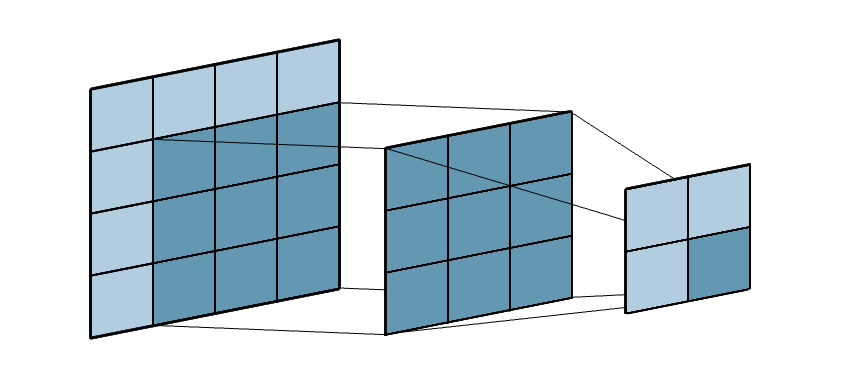
\includegraphics[width=0.5\textwidth]{images/convolution.png}
	\caption{Convolution of matrix $X$ with kernel $w$, producing $y = X\ast w$. Figure scanned from \cite{IMG:CONVOLUTION}.}
	\label{fig:convolution}
\end{figure}

\subsubsection*{Convolutional layers}
Convolutional layers take matrices with dimensions $(w_1, h_1, c_1)$ that represent input images with width $w_1$, height $h_1$ and $c_1$ channels. This matrices are convolved with $k$ filters of size $f$, producing an output matrix with dimensions $(w_2, h_2, c_2)$, with:
\begin{itemize}
	\item $r_2 = \frac{r_1 - f + 2p}{s} + 1$
	\item $c_2 = \frac{c_2 - f + 2p}{s} + 1$
	\item $d_2 = k$
\end{itemize}
where $p$ is the the amount of zero-padding used and $s$ is the value of the stride \cite{STANFORD}.

When there is a need to increase the size of the input data, typically zero-padding is used, meaning that the image is padded evenly by adding rows and columns of zeroes.
If the right amount of zero-padding is used, this type of padding is known as \textbf{same} padding, since after the convolution operation, the layer's output will keep the same spatial dimensions as its input.

On the other hand, when there is no padding applied to the input of the convolution layer, the filter window always stays at a valid position within the input matrix, producing that the output size shrinks depending on the filter size $f$. For this reason, this kind of padding is called \textbf{valid} padding.

\subsubsection*{Architecture of CNNs}

The architecture of a \glspl{cnn} varies depending on the task being performed, although they typically share:
\begin{itemize}
	\item An input layer that is a tensor with shape 
	$(n, r, c, d)$, where $n$ is the number of images to be processed, $r$ is the number of rows of pixels or image height, $c$ is the number of columns of pixels or image width, and $d$ is the image depth or number of channels.
	\item Multiple hidden layers that usually are convolutional layers that convolve their input with a set of $k$ filters producing a set of filtered images as a result that will be used as the input of the next layer.
	\item Activation layers that apply an activation function to the result of the hidden layer. In \gls{cnn}, the most commonly used activation function is \gls{relu}, since it has demonstrated to make convergence faster \cite{RELU}.
\end{itemize}

Depending on the task being carried out, the architecture can also present:
\begin{itemize}
	\item Pooling layers that shrink the image stack produced by the convolution layers. These typically consist of filters of a given size that are used to downsize the resulting matrix of the convolution layer. There are different types of pooling layers depending on the used pooling function. These usually are: max pooling and average pooling.
	\item Fully connected layers that will compute the class scores. Each neuron in these layers is connected to all the outputs of the previous layer. s
\end{itemize}


\subsection{Single image super-resolution}

\subsection{Noise reduction}